\section{Introduction}
\label{sec:al-introduction}
An Al adatom on the Al(100) surface provides an interesting system to study.
Several different low energy diffusion mechanisms have been found, including various concerted displacements of two or more atoms, in addition to the, more intuitive, hop mechanism~\cite{concerted-motion-1990, dimer-original-1999, ts-opt-2001}.
The dimer method, on which the current implementation of ridge calculations heavily depends, has been used successfully on the system~\cite{dimer-original-1999}, using the well tuned and fast embedded atom method (\fref{sec:potentials})~\cite{eam-1983, eam-1986}.
This made the system an excellent candidate for trying the newly implemented ridge method (\fref{chap:erm}, paper \ref{pap:second-order}).

\begin{SCfigure}[5.0][h]
\centering
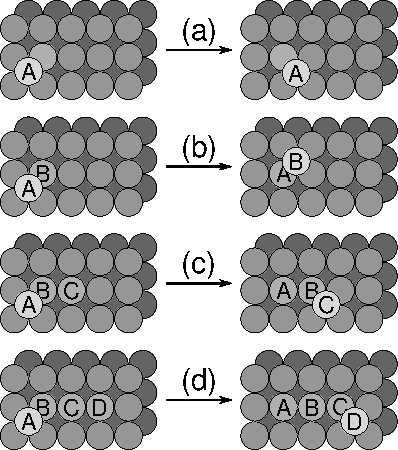
\includegraphics[width = 0.35\linewidth]{processes}
\caption{A schematic of the processes that are being considered.
(a) is the hop over a ridge.
(b) is the concerted displacement of two atoms, where the adatom, A, burrows into the surface and the surface atom, B, emerges at a different site.
(c) is the concerted displacement of three atoms.
Similarly to (b), A burrows into the surface but B does not emerge as it moves into the surface site of C, which in turn emerges at an even further site.
(d) is the concerted displacement of four atoms.
Similar to (c) but an extra surface atom, D, takes part as well and emerges still further away.
}
\label{fig:processes}
\end{SCfigure}

The obvious hop-over-ridge ($E_\text{b} = 0.372\unit{eV}$) is not the lowest energy diffusion mechanism.
Considerably lower in energy is the concerted motion of 2 atoms, where the adatom burrows into the surface to replace an atom which in turn pops out of the surface at a neighbouring site.
This mechanism has a barrier of $E_\text{b} = 0.227\unit{eV}$.
Related to the concerted 2 atom mechanism are the concerted 3 atom ($E_\text{b} = 0.426\unit{eV}$) and concerted 4 atom ($E_\text{b} = 0.413\unit{eV}$) mechanisms, where more surface atoms take part in the concerted mechanism.
These latter diffusional mechanisms are of a noticeably longer range than the hop --- and to a lesser extent the concerted 2 atom mechanism --- as the surface atom that "pops" up, does so in a more distant site.
All the processes under consideration are shown schematically in \fref{fig:processes}.

Of course, there is an incredible amount of mechanisms possible for the 385 atom system of 771 degrees of freedom\footnote{The calculational cell was composed of $2$ frozen layers and $4$ free layers of $8\times 8$ atoms with a single adatom on top. For further calculational parameters, please refer to section 3 of paper \ref{pap:second-order}.}.
However, only these lowest ones were considered for the current study as they are the most relevant when considering the real-world diffusion and present a challenging enough task for the ridge method.
The long-range concerted mechanisms are difficult to locate due to their environment being very flat, thus investigating the ridges lying close by is an interesting subject, with a high possibility of seeing low energy \sap{2}s in the vicinity of the \sap{1}s.
Furthermore, there is a clear separation in geometry between the hop mechanism on the one hand and the concerted displacements on the other, giving a similar situation as the one presented in \fref{sec:borohydrides-summary}.
